Beantwoord de onderstaande vragen voor een gelijkstroommotor waarvoor onder
meer de volgende specificaties zijn gegeven in de onderstaande tabel.

\begin{center}
    \textbf{Motor Specifications}
\end{center}

\begin{align*}
    &\text{Nominal Voltage (U\textsubscript{klem\_nom)}:} & 24 \, \text{V} \\
    &\text{Nominal Current (I\textsubscript{klem\_nom)}:} & 10.71 \, \text{A} \\
    &\text{Efficiency:} & 70\% \\
    &\text{No-load Speed (n\textsubscript{no\_load}):} & 1910 \, \text{rpm} \quad (T\textsubscript{nullast} = 0 \, \text{Nm}) \\
    &\text{Nominal Shaft Torque (T\textsubscript{as\_nom}):} & 1.0 \, \text{Nm}
\end{align*}


\begin{enumerate}
    \item [a.] \textbf{Bepaal het nominale vermogen op de as van de motor ($P_{\text{as\_nom}}$):}
    
        $P_{\text{nominaal}} = \text{Nominal Voltage} \times \text{Nominal Current} \times \text{Efficiency} = 24 \times 10,71 \times 0.70 = 179,24W$



    \item [b.] \textbf{Teken de koppeltoeren-karakteristiek van de motor. Geef duidelijk aan bij
    welke waarde de karakteristiek de verticale as snijdt en bij welke waarde de
    karakteristiek de horizontale as snijdt.}

        $T\textsubscript{stall} = \frac{U\textsubscript{klem}}{R\textsubscript{r}} \times K\textsubscript{em} = \frac{U\textsubscript{klem}}{\frac{U\textsubscript{klem}}{I\textsubscript{klem}}} \times K\textsubscript{em} = \frac{24}{\frac{24}{10,71}} \times 0,09 = 0,96 \text{ Nm}$

        $\omega_{null} = \frac{U\textsubscript{klem}}{K\textsubscript{em}} = 266,66 \text{ rad/s}$

        \begin{figure}[h]
            \centering
            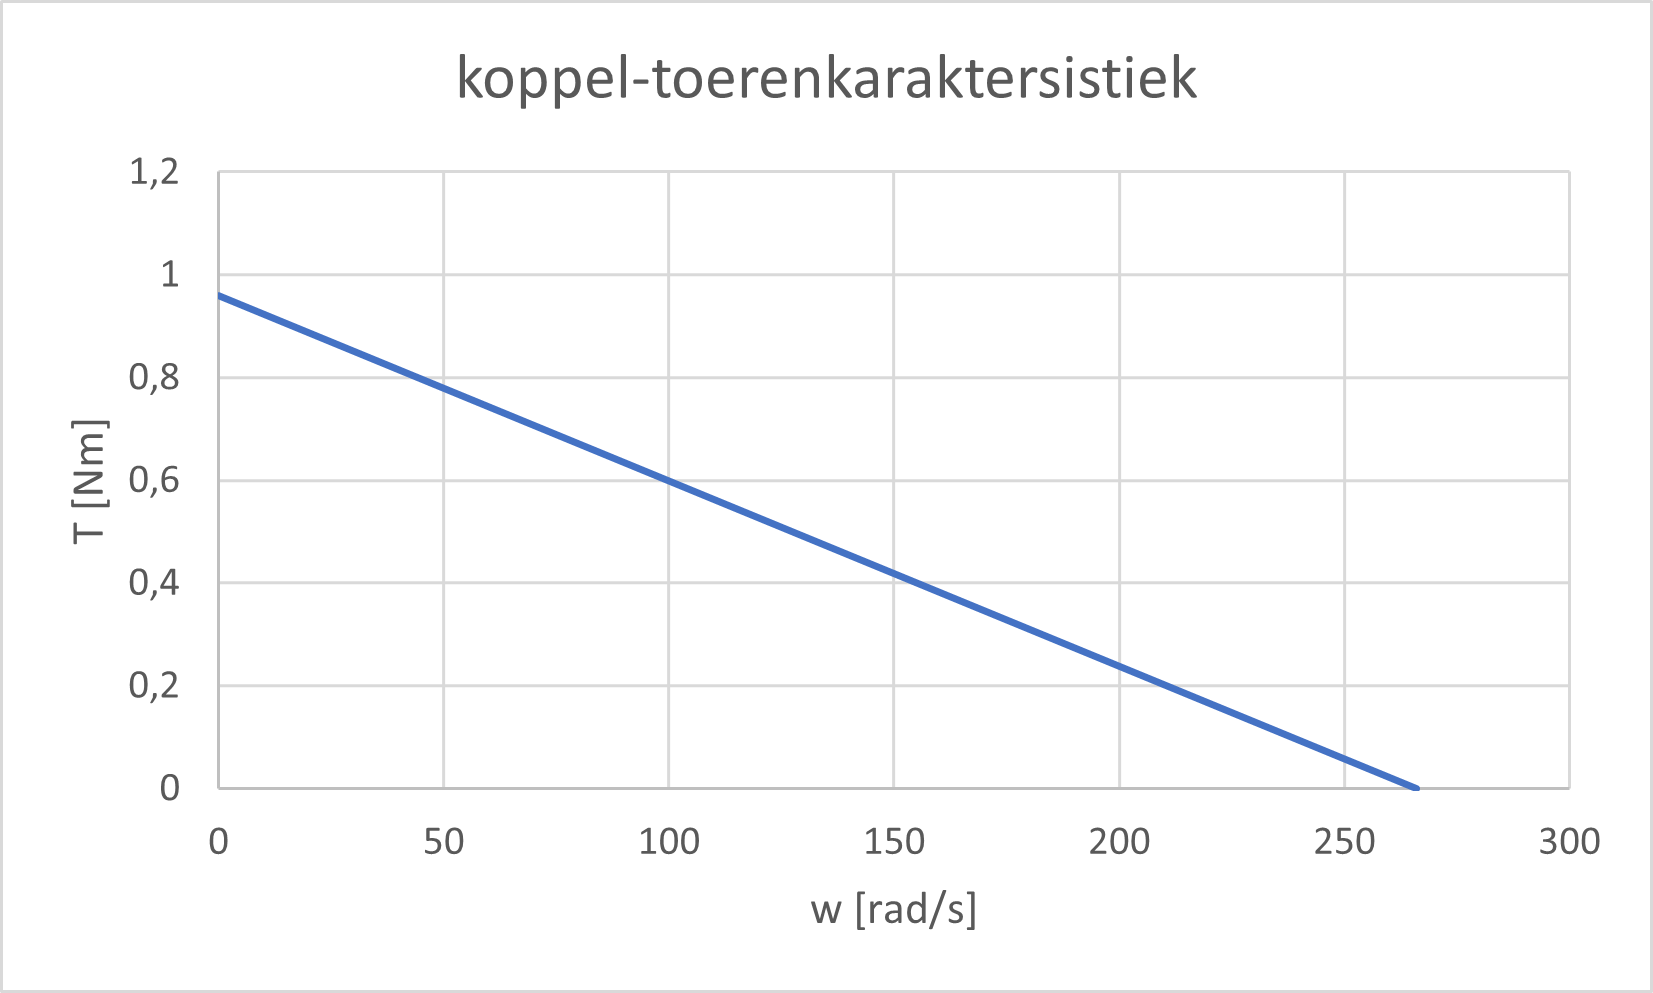
\includegraphics[scale=0.7]{koppel-toerenkarakteristiek 1b.png}
            \caption{koppel-toerenkarakteristiek}
        \end{figure}

    \item [c.] \textbf{Een belangrijke parameter van de motor is de motorconstante $K_{\text{em}}$.
    Bereken deze.}

        $K\textsubscript{em} = \frac{T\textsubscript{as}}{I\textsubscript{klem}} = \frac{1,0}{10,71} = 0,09 \text{ Nm/A}$

    \item [d.] \textbf{De motor wordt gebruikt voor het aandrijven van een toerental onafhankelijke
    last van $T_{\text{last}}$ = 200 mNm. De klemspanning van de motor is ingesteld op 24V
    Bepaal nu het werkpunt van de motor: het toerental en het koppel. Wat is bij dit werkpunt de opgenomen stroom?} 

        dit is het antwoord.

    \item [e.] \textbf{De motor wordt gebruikt voor het aandrijven van een toerental onafhankelijke
    last van $T_{\text{last}}$ = 200 mNm. Dus dat is nog dezelfde situatie als bij opgave d).
    De klemspanning wordt nu echter 12V.
    Bepaal nu weer het werkpunt van de motor: het toerental en het koppel.
    Wat is bij dit werkpunt de opgenomen stroom?}

        dit is het antwoord.

\end{enumerate}
